%\documentclass[xcolor=dvipsnames]{beamer}
\documentclass[xcolor=dvipsnames, notes]{beamer}

\usetheme{Warsaw}

\usepackage{inputenc}
\usepackage{amsmath}
\usepackage{amsthm}
\usepackage{graphicx}
%\usepackage{geometry}
\usepackage{tasks}
\ifodd\textwidth
  \addtolength{\textwidth}{1sp}
\fi


\newcommand{\po}{\textcolor{BlueViolet}{po}}
\newcommand{\ppo}{\textcolor{BlueViolet}{ppo}}
\newcommand{\rf}{\textcolor{Green}{rf}}
\newcommand{\rfe}{\textcolor{Green}{rfe}}
\newcommand{\ws}{\textcolor{BurntOrange}{ws}}
\newcommand{\fr}{\textcolor{RubineRed}{fr}}
\newcommand{\com}{\textcolor{BurntOrange}{com}}
\newcommand{\barr}{\textcolor{Apricot}{bar}}

\newcommand{\ghb}{\textcolor{NavyBlue}{ghb}}

\newcommand{\ato}{\textcolor{RoyalPurple}{ato}}


\newcommand{\co}{\textcolor{BurntOrange}{co}}
\newcommand{\mo}{\textcolor{Red}{mo}}
\newcommand{\hbsc}{\textcolor{NavyBlue}{hbsc}}
\newcommand{\xhb}{\textcolor{NavyBlue}{xhb}}
\newcommand{\rfi}{\textcolor{Green}{rfi}}
\newcommand{\brf}{\textcolor{Green}{brf}}
\newcommand{\jhb}{\textcolor{NavyBlue}{jhb}}
\newcommand{\jmo}{\textcolor{Red}{jmo}}

\title{Fast RMW for TSO: Semantics and Implementation}
\subtitle{Bhargava Rajaram, Vijay Nagarajan, Susmit Sarkar, Marco Elver}

\author{Presented by \\ Akshay Gopalakrishnan}

\begin{document}

    \begin{frame}

        \maketitle

    \end{frame}

    \begin{frame}{Introduction}

        \begin{itemize}
            \item Read-Modify-Write (RMW) semantics is too strong for TSO.  
            \item RMWs for TSO also implies a write buffer flush beforehand, which is very expensive.
            \item The write buffer flush is often not required while using RMWs for concurrent algorithms. 
            \item Examining the possible compiler mappings from C11 to TSO for Dekker's algorithm exposes the unnecessary strong semantics of RMW.
            \item Weakening such strong RMW semantics for TSO is beneficial for performance and can retain correctness of concurrent algorithms.
        \end{itemize}

    \end{frame}

    \begin{frame}{What the paper is about}

        \begin{itemize}
            \item Formally specifying weaker semantics for RMW - dividing RMW usage into 3 atomicity constraints.
            \item Showing which of these variants of RMW work for different implementation of Dekker's Algorithm to maintain mutual exclusion and deadlock freedom.
            \item Discussing and proposing implementation of such RMWs in hardware that enforces TSO semantics.
        \end{itemize}

    \end{frame}


    %Give the 3 variant implementations of DEkker's algorithm as per C11 mappings to RMWs.
    \begin{frame}{Model looking at: Total Store Order (TSO)}

        Intuitively:
        \begin{itemize}
            \item Every CPU has a FIFO write buffer.
            \item Writes issued by CPU are committed to respective buffers. 
            \item Reads issued by CPU first checks if the respective buffer has a write to the same memory. If not, it takes the value from main memory.
            \item Buffers can be flushed randomly to main memory or can be forced by MFENCE instruction or read-modify-writes (RMW).
        \end{itemize}


    \end{frame}


    \begin{frame}{Dekker's Algorithm: 3 variants using RMW}

        \begin{figure}
            \makebox[\textwidth][c]{
                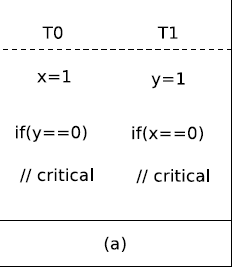
\includegraphics[scale=0.7]{DekkerC.png}
            }
        \end{figure}

        \begin{figure}
            \makebox[\textwidth][c]{
                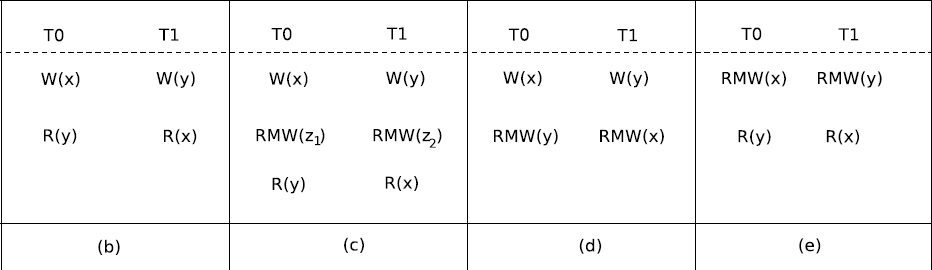
\includegraphics[scale=0.7]{Dekker_Axiomatic.png}
            }
        \end{figure}

        %Explain why not use MFENCES
        %Perhaps it is just the expense of using MFENCE 

    \end{frame}

    \note{
        One might ask why not use MFENCE when implementing Dekker's algorithm in TSO model.
        The possible reasons for not doing so are the following:
        \begin{itemize}
            \item RMW itself includes fence semantics in the TSO semantics.
            \item (c) can definitely be avoided as it involves an RMW which is not required. 
            \item (d) and (e) combines the fence and the memory operation, but also involves an extra memory event.
            \item It must be that RMW implementation allows the combination of memory operation and fence to be faster than a separate fence followed by a separate memory event.
            \item Hence, such an implementation makes sense.
        \end{itemize}

    }

    %Introduce the intuition behind each RMW atomicity semantics, what it enforces and what it does not.
    \begin{frame}{Intuition: Original RMW - Type 1 Atomicity}

        No memory event can happen in between the RMW. 
        \begin{itemize}
            \item First flush all pending writes to main memory.
            \item Then perform the RMW read part.
            \item Then perform the RMW write part. 
            \item Commit this write to memory.
            \item We are done. 
        \end{itemize}
    
    \end{frame}

    \note{
        The default view of read-modify-write events is that no other memory access is supposed to take place or be serviced by the system until this is done.
        Think of it as taking a global lock and then performing a flush, followed by a read and a write committed to memory. 
    }

    \begin{frame}{Intuition: Weakening RMW - Type 2 Atomicity}

        No conflicting memory events can happen in between the RMW.
        \begin{itemize}
            \item If write-buffer has conflicting events, only then perform a buffer flush until that write is committed.
            \item Then perform the RMW read part.
            \item In between any number of non-conflicting memory accesses can occur.
            \item Then perform the RMW write part.
            \item Commit this write to memory.  
        \end{itemize}

    \end{frame}


    \begin{frame}{Intuition: Further weakening RMW - Type 3 Atomicity}

        No conflicting writes can happen in between the RMW.
        \begin{itemize}
            \item Same as Type 2 atomicity. 
            \item Except in between any number of conflicting read accesses can also occur.
        \end{itemize}

    \end{frame}

    \note{

        In truth, one may not require such strong guarantees from RMW, otherwise the point of MFENCE is sort of debatable: why not use RMW everywhere and ditch the MFENCE entirely??
        Hence, it is rather better to have a separation and not entirely keep the fence semantics as part of RMW.
        Thus, these weakenings in what RMW should ensure. 

    }


    %Semantics of TSO
    
    \begin{frame}{Towards Axiomatic Formulation: Preliminaries}

        \begin{itemize}
            \item $\po$ - Intra-thread syntactic order.
            \item $\ppo$ - Order preserved by TSO ($\po \setminus [W];\po;[R]$)
        \end{itemize}

        \begin{itemize}
            \item $\rf$ - Reads-from
            \item $\rfe$ - Reads-from external 
            \item $\ws$ - Write serialization (coherence order)
            \item $\fr$ - From-reads (reads-before)
            \item $\barr$ - Barrier (MFENCE)
        \end{itemize}

        
    \end{frame}

    \begin{frame}{Axiomatic model without RMW}

        \begin{itemize}
            \item $\com = \rfe \cup \ws \cup \fr$.
            \item $\ghb = (\com \cup \ppo \cup \barr)*$. 
        \end{itemize}

        Axioms of TSO (without RMWs)
        \begin{itemize}
            \item $\ghb$ acyclic.
            \item $\com \cup \po_{loc} \cup \barr$ acyclic (uniproc).
        \end{itemize}

    \end{frame}

    \note{

        To be honest, the two axioms of TSO can be potentially combined. 
        The TSO model by Viktor and Ori in terms of irreflexivity constraints seem to be much simpler in understanding what the axioms mean.
        In some sense, the individual relations here do make sense.
        But the uniproc axiom seems unnecessary; one can instead define $\ppo$ to be $\po$ that preserves $\po_{loc}$ totally. 
        Then the axiom would just be one acyclicity.

        Perhaps for the sake of proofs it is not done so.

    }

    \begin{frame}{Adding RMW}

        \begin{itemize}
            \item RMW events ($R_{a}$, $W_{a}$ together) introduce additional memory ordering constraints.
            \item These are represented by $\ato$ (atomically induced orderings).
            \item The indicate which memory events cannot take place between the read and write part of RMW. 
            \item Eg: Some memory operation $M$ has to take place after an RMW gives ($[W_{a}];\ato;[M]$).
            \item The above also implies $[R_{a}];\ato;[M]$.
        \end{itemize}

        Modified axiom of TSO now involves new $\ghb = (\com \cup \ppo \cup \barr \cup \ato)* $.
        
    \end{frame}

    \note{

        Adding RMW just involves from the axiomatic perspective, a new partial order between already existing events and RMW events. 
        This relation is what will play a role in defining the semantics of RMW. 
        The different variants of RMW semantics revolve around this new partial order called $\ato$.
        What I find a bit disappointing from the paper is that this is not specified properly and hence leads to confusion.

        Instead the paper uses previous $\ghb$ definition to define semantics of each RMW.
        It then uses these definitions to derive $\ato$ between the events, specified as lemmas. 
        But the lemmas need to be more specific to $\ato$ and not the combined memory orderings.

    }

    %Semantics of different RMW based on their atomicity types
    \begin{frame}{Formal: Original RMW: Type 1}
        
        Reads/Writes to any address cannot appear in between the RMW.
        \begin{align*}
            \forall M . [M];\ghb;[R_{a}] \vee [W_{a}];\ghb;[M].
        \end{align*}

        \begin{lemma}
            A type 1 RMW placed between a write $W$ and read $R$ in a thread enforces: 
            \begin{align*}
                [W];\ato;[R_{a}] \wedge [W_{a}];\ato;[R] \wedge [W];\ato;[R].    
            \end{align*}
        \end{lemma}


    \end{frame}

    \note{

        Note that this is a thread-local property.
        The $\ghb$ around one of the atomic memory events imply an $\ato$ on the other. 
        Simply using $\ppo$ and type 1 RMW is enough to prove. 
    }

    %Explaining variants of Dekker's that work
    \begin{frame}{Visiting Dekker's: Type 1 atomicity}

        \begin{figure}
            \makebox[\textwidth][c]{
                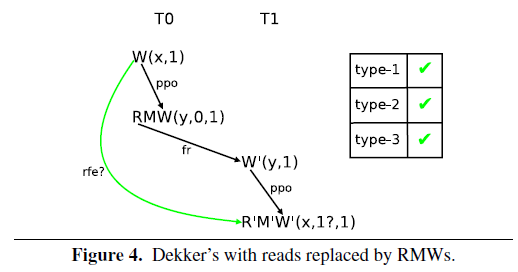
\includegraphics[scale=0.7]{Dekker_Read_RMW.png}
            }
        \end{figure}




    \end{frame}



    \begin{frame}{Formal: Weakening RMW: Type 2}

        Reads/Writes to the same address cannot appear in between the RMW.
        \begin{align*}
            \forall M(x) . [M(x)];\ghb;[R(x)_{a}] \vee [W(x)_{a}];\ghb;[M(x)].
        \end{align*}

        \begin{lemma}
            A type 2 RMW placed between a write $W$ and read $R$ in a thread enforces: 
            \begin{align*}
                \neg [R_{a}];\ghb;[W] \wedge \neg [R];\ghb;[W_{a}].    
            \end{align*}
        \end{lemma}

    \end{frame}
    
    \note{

        Note firstly that this is a thread-local property. 
        The intuition is that it even if any read or write occur in between the type 2 RMW, it will NOT be part of the global memory order.
        We must note that $\ghb$ is actually related to write buffer flushes, which enforce certain serialization order of writes. 
    }

    %Explaining variants of Dekkers that work / dont
    \begin{frame}{Visiting Dekker's: Type 2 atomicity}

        \begin{figure}
            \makebox[\textwidth][c]{
                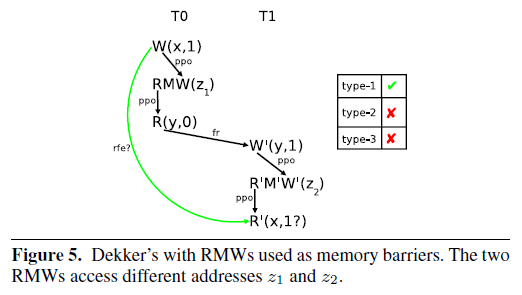
\includegraphics[scale=0.7]{Dekker_Barrier_RMW.png}
            }
        \end{figure}


    \end{frame}



    \begin{frame}{Formal: Further Weakening RMW: Type 3}

        Writes to the same address cannot appear in between the RMW.
        \begin{align*}
            \forall W(x) . [W(x)];\ghb;[R(x)_{a}] \vee [W(x)_{a}];\ghb;[W(x)].
        \end{align*}

        \begin{lemma}
            A type 3 RMW placed between a write $W$ and read $R$ in a thread enforces: 
            \begin{align*}
                \neg [R_{a}];\ghb;[W].    
            \end{align*}
        \end{lemma}

    \end{frame}

    \note{

        The intuition again is that a write could take place in between, but it will not be part of a global memory order. 
        But the read can potentially be part of it, when it occurs in between them.
        In between them is more to say that any read outside can also perform its read before the write is actually performed by the RMW.

    }

    %Explaining variants of Dekkers that work / dont
    \begin{frame}{Visiting Dekker's: Type 3 atomicity}

        \begin{figure}
            \makebox[\textwidth][c]{
                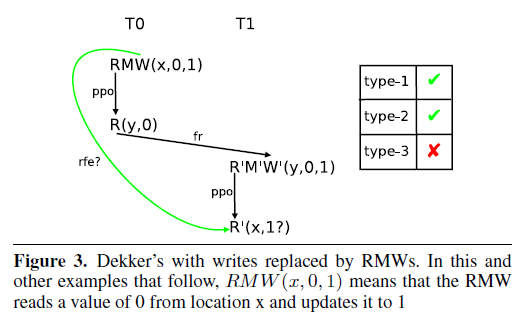
\includegraphics[scale=0.7]{Dekker_Write_RMW.png}
            }
        \end{figure}


    \end{frame}


    %Towards implementation:
    \begin{frame}{Implementation: Original RMW: Type 1}

    \end{frame}
    
    \begin{frame}{Implementation: Weakening RMW: Type 2}

    \end{frame}
    
    \begin{frame}{Implementation: Further Weakening RMW: Type 3}

    \end{frame}

    %Final works and recap
    \begin{frame}{Recap}

    \end{frame}


    \begin{frame}{Conclusion}

    \end{frame}

    
    \note{

        Honestly, this paper lacks flow of intuition. 
        The lemmas placed and stated have no purpose stated before to emphasize its need.
        It is my understanding that these lemmas are actually not required to be honest. 
        Perhaps just Lemma 1 suffices, but even that can be elided as we can simply use the definition of type 1 RMW.

        What the authors forget to convey, is that much of the results are actually local.
        Which means, lets say for type 2 RMW, there are non-conflicting read/writes that could intervene from other threads.
        This is not much emphasized, and Lemma 2 actually makes this worse to understand, as it is a thread-local property.

        The connection of the Lemmas to the implementation is also not so clear, but my intuition says it potentially plays a role. 
        Perhaps the authors could do a better job at that.
        The results surely are interesting and useful to consider for performance and as an optimization of RMW, but the presentation lacks clarity and intuition.

    }

\end{document}
